\section{Problema 1}

\subsection{Introducción}
%\textit{Acá va la explicación de las ideas de forma clara, sencilla, estructurada y concisa. Se puede usar lenguaje coloquial o pseudocódigo, o combinar ambas herramientas. Esto debe ser lo suficiente para el desarrollo de los otros puntos, pero no excesivo.}\\

La idea detrás de nuestra solución para el Problema 1 involucra recorrer la lista de precios una sola vez. Logramos concluir que podíamos separar el problema de la lista entera en sublistas crecientes, ya que no nos interesa cuando un precio cualquiera precede a otro precio inferior a él. De esta forma, creamos una variable que guarda la mejor ganancia a medida que se va avanzando. Dicha ganancia máxima empieza en 0 y se la pisa con la primer ganancia calculada, que luego es pisada nuevamente por las ganancias mejores que ella en caso de haberlas.\\
\\
\indent La ganancia se calcula de la siguiente forma:
\begin{itemize}
	\item Se recorre el arreglo de precios. Se setea la primera posición como posición de compra y de venta.
	\item En cada iteración se guarda la ganancia actual según el último precio de compra y el precio de venta de esa posición.
	\item En cada posición del mismo se mira si es mayor o menor que la anterior. Si es mayor, se toma como nuevo precio de venta, y la resta entre el precio de venta y el de compra es la ganancia de la sublista actual. Si es menor indica el inicio de una sublista nueva. Se toma como nuevo precio de compra y se guarda la ganancia en \textit{ganancia máxima} en caso de ser mayor que la ganancia máxima anterior.
\end{itemize}

\indent Observación: Por comodidad, cuando levantamos el archivo, lo pasamos a un arreglo, que es el que se le pasa a la función para resolver el costo.\\

\subsection{Complejidad}
\indent Para analizar la complejidad del algoritmo planteado anteriormente, utilizaremos el siguiente pseudocódigo:

\begin{verbatim}
for ( 1 <= i < cantDias ){
   if (precios[i] < min)
      min = precios[i]
      max = precios[i]
   if (precios[i] > max) max = precios[i]
   
   gananciaActual = max - min
   if (gananciaActual > gananciaMax) gananciaMax = gananciaActual
return gananciaMax;
\end{verbatim}

\indent Básicamente, nuestro algoritmo recorre linealmente el arreglo de los días y va guardando la ganancia máxima, que luego es el valor devuelto.\\
\indent Para empezar a analizar la complejidad, podemos notar que ciclamos por todas las posiciones del arreglo una sola vez. Esto quiere decir que la complejidad que tenemos va a ser de $O(n)$ por el costo del cuerpo del $for$, considerando a n, como el tamaño del arreglo (cantidad de días).\\
\indent Una vez analizado el ciclo, podemos meternos de lleno con el cuerpo del mismo y ver que es lo que pasa adentro.\\
\indent Tenemos 3 comparaciones y varias asignaciones para tener en cuenta su complejidad. Para ver el costo de estas operaciones recurrimos a la documentación de $Java$ y comprobamos que tanto las comparaciones de enteros, como las indexaciones en arreglos, toman un tiempo constante. Visto esto, podemos analizar el peor caso del cuerpo del ciclo. Tenemos 2 casos disjuntos a tener en cuenta:

\begin{itemize}
 \item precios[i] $<$ min: el valor del precio del producto en el día $i$ es menor al mínimo anterior.
 \item precios[i] $>$ max: el valor del precio del producto en el día $i$ es mayor al máximo anterior.
\end{itemize}

\indent Se puede ver claramente que estos casos son disjuntos porque al comparar por menor y mayor (nunca por igual) no puede pasar que un numero cumpla ambas condiciones.\\
\indent La comparación por menor al mínimo, lleva a tener que hacer 2 indexaciones en el arreglo y 2 asignaciones de enteros, cuando la comparación de mayor al máximo lleva a tener 1 sola indexación y una asignación. Por lo tanto consideramos el peor caso, como un arreglo estrictamente decreciente, adonde se cumple siempre la guarda del primer $if$. Como estamos usando el modelo uniforme, en este caso tenemos $O(1)$ + $O(1)$ + $O(1)$ + $O(1)$ que por el álgebra de ordenes, es $O(1)$. \\                                                   
\indent Luego hacemos una resta entre 2 enteros, nuevamente $O(1)$ y otra asignación. Si se cumple la guarda del ultimo $if$, nuevamente hacemos una comparación y una asignación, por lo tanto seguimos trabajando en tiempo constante.\\
\indent Por lo visto anteriormente, podemos decir que la complejidad del cuerpo del ciclo es $O(1)$ y como este ciclo se ejecuta $n$ veces, concluimos que la complejidad total del algoritmo es $O(n)$.\\


\subsection{Analisis del tiempo de ejecución}

\begin{figure}[h]
\centering                                                       
        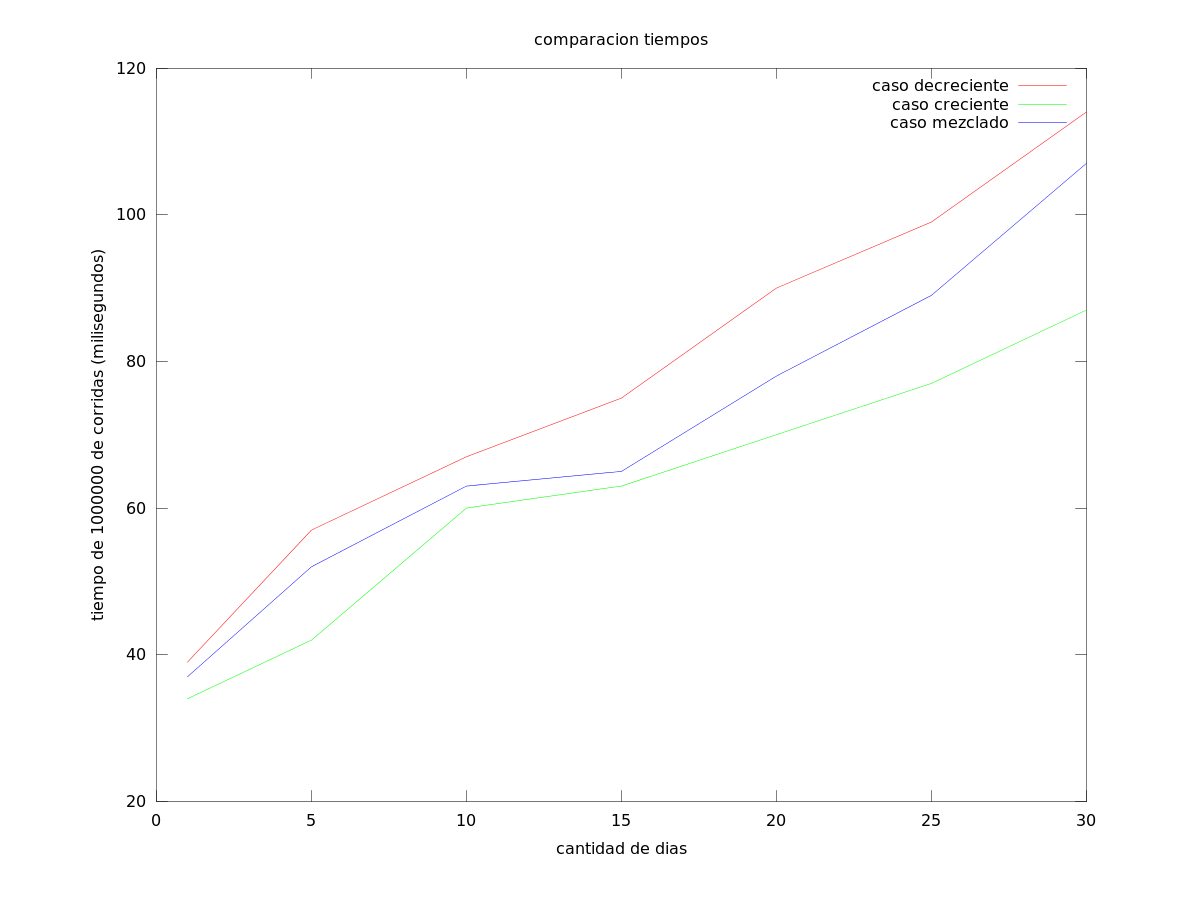
\includegraphics[width=340pt]{./figs/p1Tiempos.png}
\end{figure}





